\chapter{Badania skuteczności detekcji obiektów YOLOv8n}
Rozdział ten opisuje autorskie testy dokładności detekcji obiektów w zależności od różnych czynników. Testowanym zadaniem jest dokładność klasyfikacji obiektów. Nie zaimplementowano testów dokładności dla lokalizacji przestrzennej, ponieważ nie jest ona priorytetem w niniejszym systemie. Uznano, iż jakościowe stwierdzenie możliwości lokalizacji w fazie tworzenia systemu jest wystarczające, a efekt uznano za zadowalający. 

Zaimplementowane dwa testy skuteczności klasyfikacji to:
\begin{enumerate}
    \item Test dokładności pojedyńczej klasy na przykładzie klasy \emph{człowiek} (ang. \emph{person}). 
    \item  Test poziomu generalizacji modelu dla różnych wariantów obiektu wchodzących w skład tej samej klasy. Analiza przeprowadzona na przykładzie klasy \emph{krzesło} (ang. \emph{chair}) i użytych wariantów: krzesło kuchenne, krzesło gamingowe (dalej nazywane fotelem). 
\end{enumerate}
W obu testech detektor był skonfigurowany, aby zwracać tylko wyniki zawierające obiekty klas \emph{człowiek} i \emph{krzesło}. Ponadto, każdy test używa filmów z tego samego zbioru nagrań. Dla każdego nagrania wygenerowano pewne metryki, które są wykorzystywane do analizy oraz wyznaczania kolejnych metryk już w konkretnym teście. Oba testy sprawdzają również skutecznośc detektora dla różnych wartośći progu ufności. Wspomniane metryki zostały więc wygenerowane dla każdej wartości progu ufności objętej testem. Wartość progu sprawdzono od $0.00$, aby następnie rosnąć co interwał $0.01$, aż do maksymalnej wartości $1.00$. Daje to łącznie sto jeden sprawdzonych wartości. Generacje metryk zaprogramowano jako test odizolowanego detektora od reszty systemu, ze względu na łatwość i czytelność implementacyjną oraz brak zależności dokładności detekcji od czynników systemowych (w przeciwnieśtwie do szybkośći).  

Biorąc pod uwagę tę strukturę, rodział ten wpierw porusza kwestie współdzielone przez oba testy w sekcji \ref{sec:test-wspoldzielony}, a następnie opisuję dalszą analize w sekcjach \ref{sec:test-1} i \ref{sec:test-2}.
 
Uwaga dotycząca zamieszconych rysunków: w rysunkach przedstawiających człowieka twarz została zamazana.


\section{Przygotowanie danych do testów}
\label{sec:test-wspoldzielony}
\subsection{Żródło wideo}
\label{sec:zrodlo_wideo}
Źródło wideo to nagrane w domowych warunkach, autorskie, krótkie filmy. Filmy nagrano na kamerze o rozdzielczości 640x480 pikseli. Obiektyw kamery jest statycznie usytuowany w tej samej lokalizacji dla każdego filmu i skierowany na wejście do pomieszczenia, w którym znajduje się kamera. Wygląd pomieszczenia przedstawiono na rysunku \ref{fig:test-dokladnosc-scena}.

\begin{figure}[H]
    \centering
    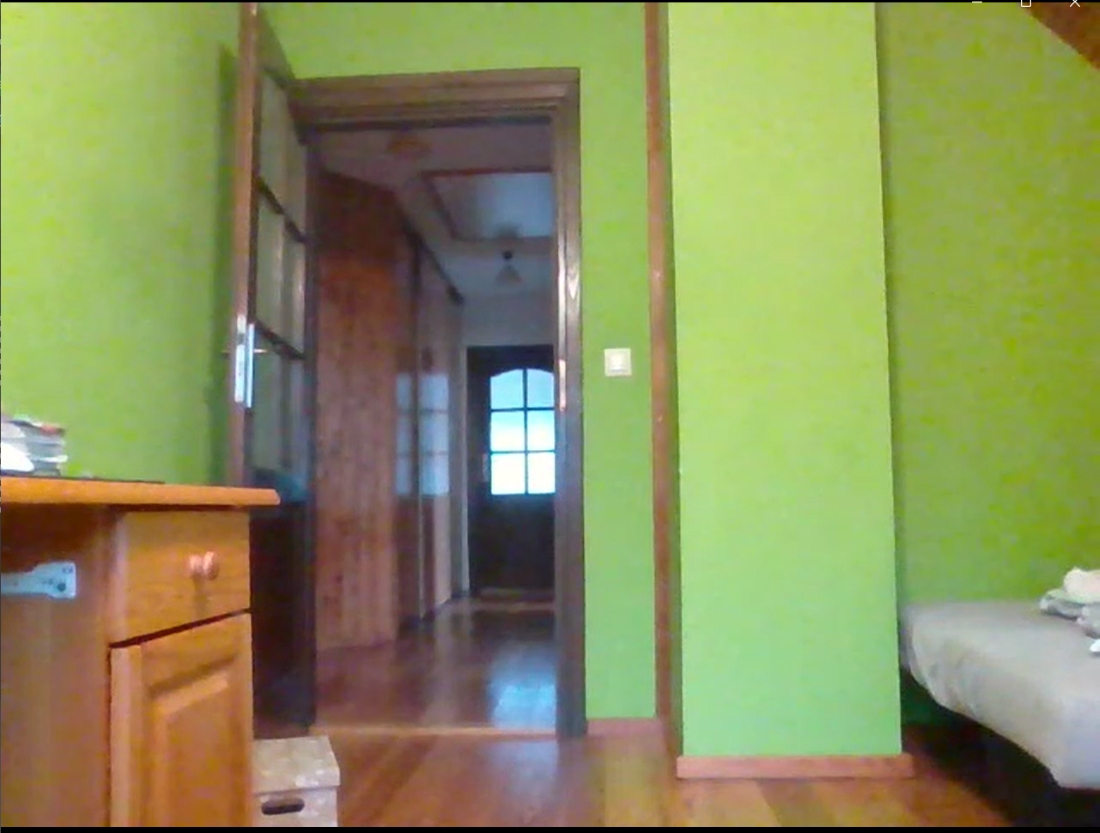
\includegraphics[width=\linewidth]{r_test_dokładności/vid_pics/1_1.jpg}
    \caption{Pomieszczenie, w którym nagrano filmy.}
    \label{fig:test-dokladnosc-scena}
\end{figure}

\begin{figure}[H]
    \centering
    \begin{minipage}{0.32\textwidth}
        \centering
        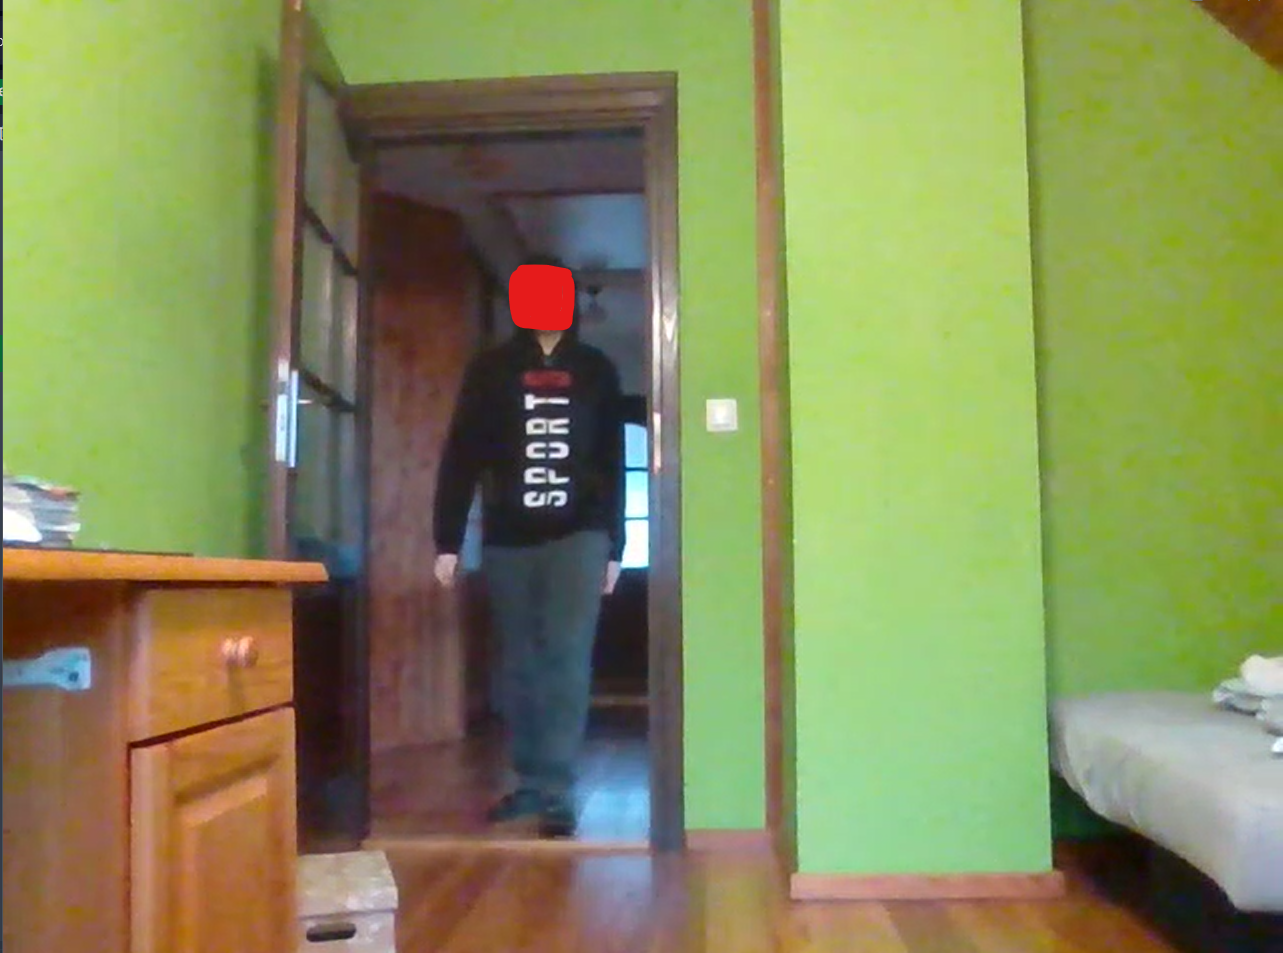
\includegraphics[width=\linewidth]{r_test_dokładności/vid_pics/1_2.png}
        \caption{Klatka filmu z człowiekiem.}
    \end{minipage}\hfill
    \begin{minipage}{0.32\textwidth}
        \centering
        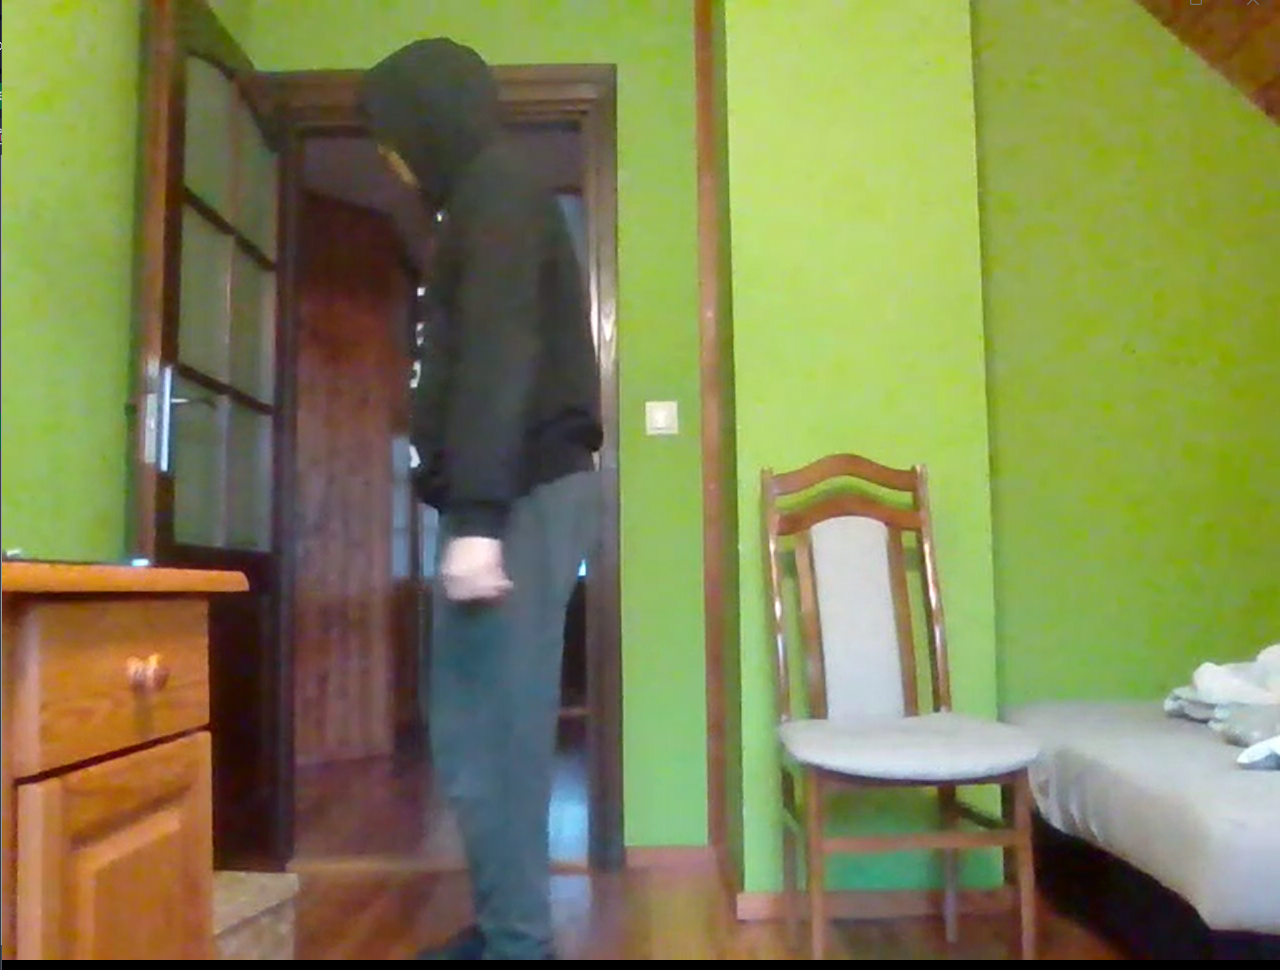
\includegraphics[width=\linewidth]{r_test_dokładności/vid_pics/1c_2.png}
        \caption{Klatka filmu z człowiekiem i krzesłem.}
    \end{minipage}\hfill
    \begin{minipage}{0.32\textwidth}
        \centering
        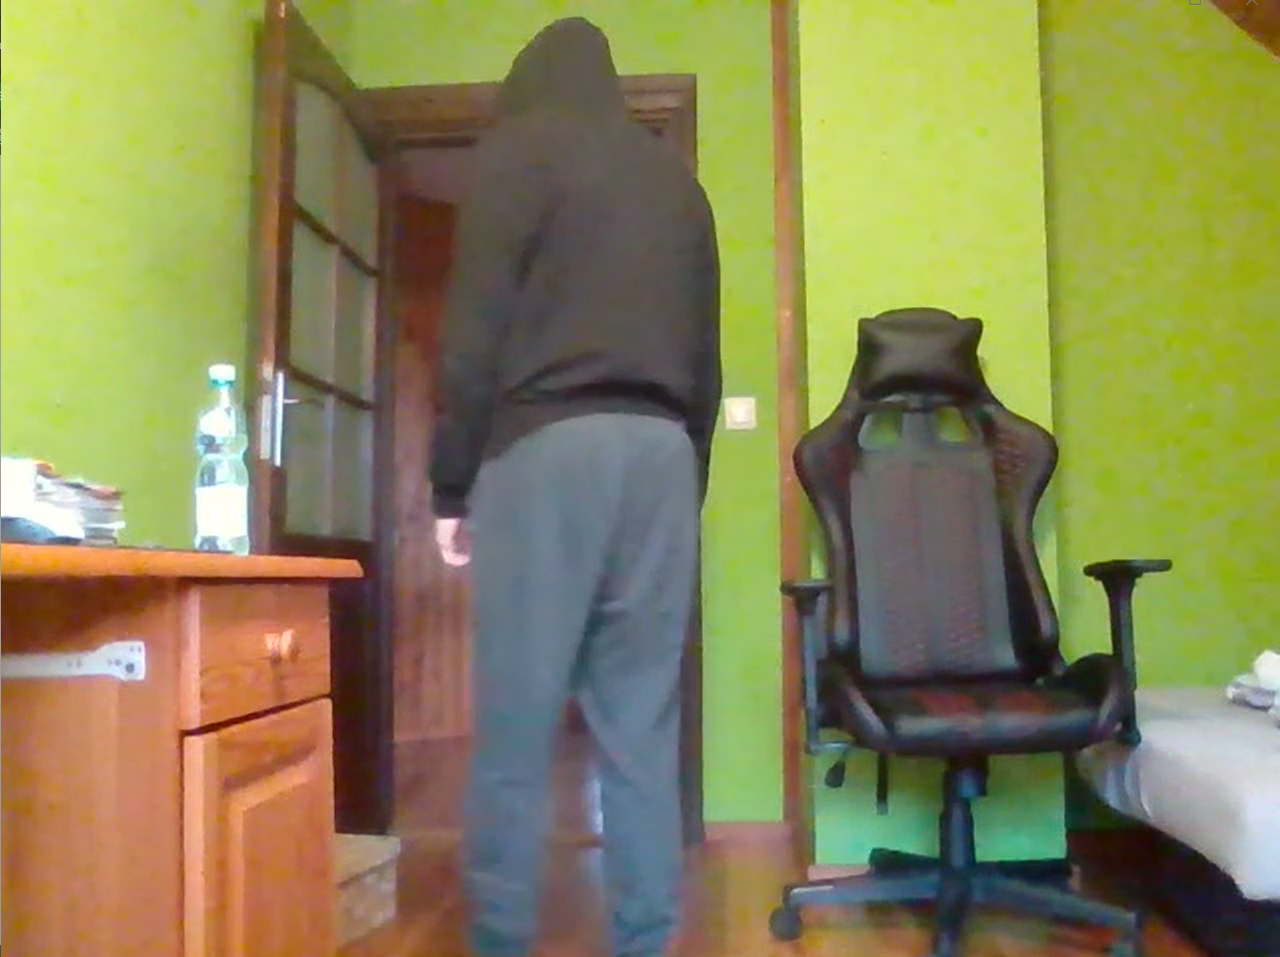
\includegraphics[width=\linewidth]{r_test_dokładności/vid_pics/1g_2.png}
        \caption{Klatka filmu z człowiekiem i fotelem.}
    \end{minipage}
    \caption{Prezentacja użytych obiektów.}
    \label{fig:all_objects}
\end{figure}
Filmy można podzielić na trzy kategorie ze względu na różne obecne w nim obiekty (wizualizacja objektów: rysunek \ref{fig:all_objects}):
\begin{itemize}
    \item człowiek
    \item człowiek, krzesło
    \item człowiek, fotel
\end{itemize}
Krzesło oraz fotel, z perspektywy filmów, są obiektami statycznymi. Przez całą długość filmu są umieszczone w jednej lokalizacji, a inne obiekty nie wchodzą z nimi w fizyczną interakcję.
Natomiast człowiek jest obiektem ruchomym. Jest on nieobecny przez pierwszą część każdego filmu. W drugiej części przekracza próg pomieszczenia, zbliża się do pewnego punktu widocznego w obiektywie, a pod koniec filmu wykonuje jeden pełen obrót wokół własnej osi. 

Należy podkreślić kilka istotnych kwestii dotyczących nagranych filmów:
\begin{itemize}
    \item Obecne obiekty nie wchodzą ze sobą w interakcję --- człowiek podczas ruchu nie zasłania konturów krzesła ani fotela.
    \item Generacja danych do testów nie odbywała się na każdej klatce nagranego filmu. Użyto tylko klatek, na których widoczne są pełne kontury obiektów. Pełny kontur człowieka pojawia się w momencie przekroczenia progu wejścia do pomieszczenia. W związku z powyższym, wykorzystano dwie sekcje każdego filmu: sekcję, w której człowiek był całkowicie nieobecny oraz sekcję od momentu przekroczenia progu.
\end{itemize}

Dla każdej kategorii filmu nagrano cztery warianty z różnym poziomem oświetlenia w pomieszczeniu, co daje łącznie dwanaście plików wideo do analizy. Wizualne różnice między poziomami przedstawiono na rysunku \ref{fig:person_grid} (człowiek), rysunku \ref{fig:chair_grid} (człowiek, krzesło) oraz rysunku \ref{fig:game_grid} (człowiek, fotel). 
Dla każdego filmu, korzystając z modelu przestrzeni barw HSV, obliczono średnią jasność oraz nasycenie. Wartości te zaprezentowano w tabeli \ref{tab:saturation-value-table}. Obliczenia polegały na wyznaczeniu średniej wartości jasności i nasycenia dla każdej klatki obrazu na podstawie wszystkich pikseli. Następnie wyznaczono średnią z uzyskanych wartości dla wszystkich klatek w filmie.
\begin{table}[H]
    \centering
    \caption{Jasność i nasycenie dla każdego nagranego filmu.}
    \begin{tabular}{|c|c|c|c|}
    \hline
    Nr sceny:          & Obecne obiekty    & Jasność & Nasycenie \\ \hline
    \multirow{3}{*}{1} & człowiek          & 152.73  & 107.3     \\ \cline{2-4} 
                       & człowiek, krzesło & 149.92  & 119.07    \\ \cline{2-4} 
                       & człowiek, fotel   & 152.68  & 111.47    \\ \hline
    \multirow{3}{*}{2} & człowiek          & 134.64  & 93.48     \\ \cline{2-4} 
                       & człowiek, krzesło & 139.14  & 90.71     \\ \cline{2-4} 
                       & człowiek, fotel   & 133.77  & 83.29     \\ \hline
    \multirow{3}{*}{3} & człowiek          & 41.59   & 123.48    \\ \cline{2-4} 
                       & człowiek, krzesło & 38.91   & 132.31    \\ \cline{2-4} 
                       & człowiek, fotel   & 38.12   & 124.31    \\ \hline
    \multirow{3}{*}{4} & człowiek          & 25.47   & 90.92     \\ \cline{2-4} 
                       & człowiek, krzesło & 25.3    & 100.8     \\ \cline{2-4} 
                       & człowiek, fotel   & 24.88   & 108.5     \\ \hline
    \end{tabular}
    \label{tab:saturation-value-table}
    \end{table}
\begin{figure}[H]
    \centering
    \begin{minipage}{0.45\textwidth}
        \centering
        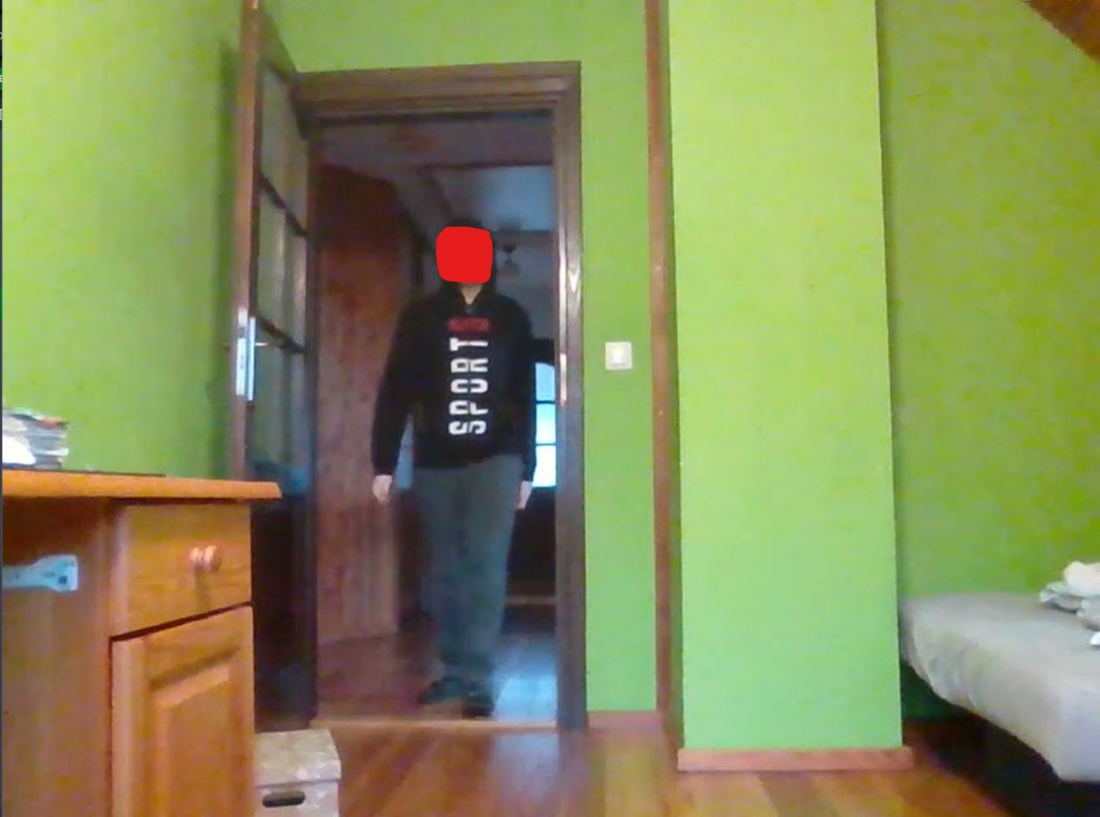
\includegraphics[width=\linewidth]{r_test_dokładności/vid_pics/1_2.jpg}
    \end{minipage}\hfill
    \begin{minipage}{0.45\textwidth}
        \centering
        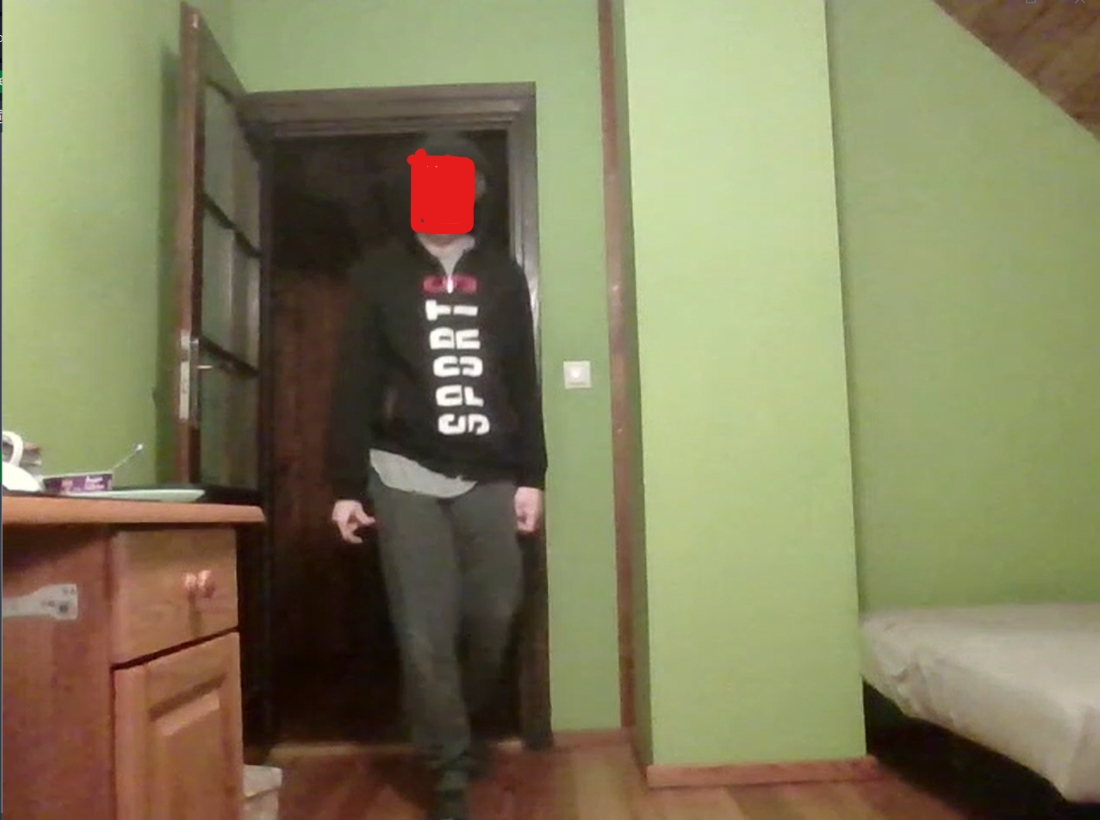
\includegraphics[width=\linewidth]{r_test_dokładności/vid_pics/2_2.jpg}
    \end{minipage}
    \vskip\baselineskip
    \begin{minipage}{0.45\textwidth}
        \centering
        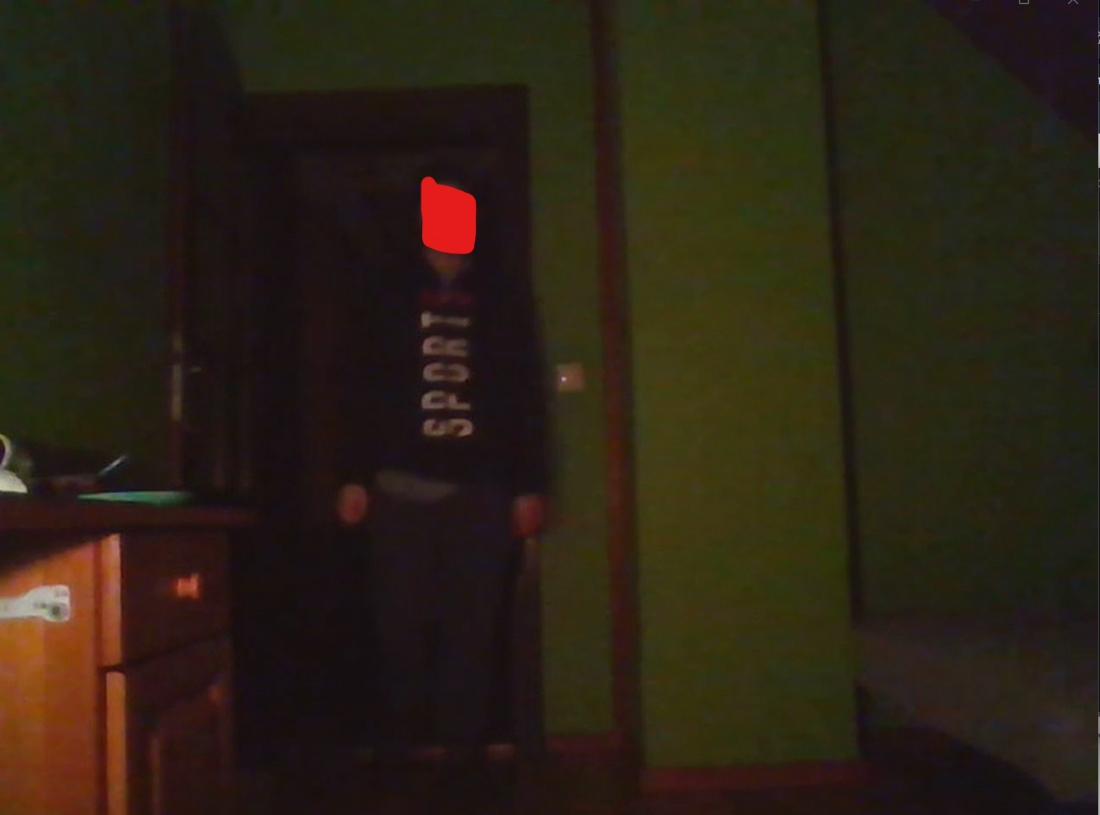
\includegraphics[width=\linewidth]{r_test_dokładności/vid_pics/3_2.jpg}
    \end{minipage}\hfill
    \begin{minipage}{0.45\textwidth}
        \centering
        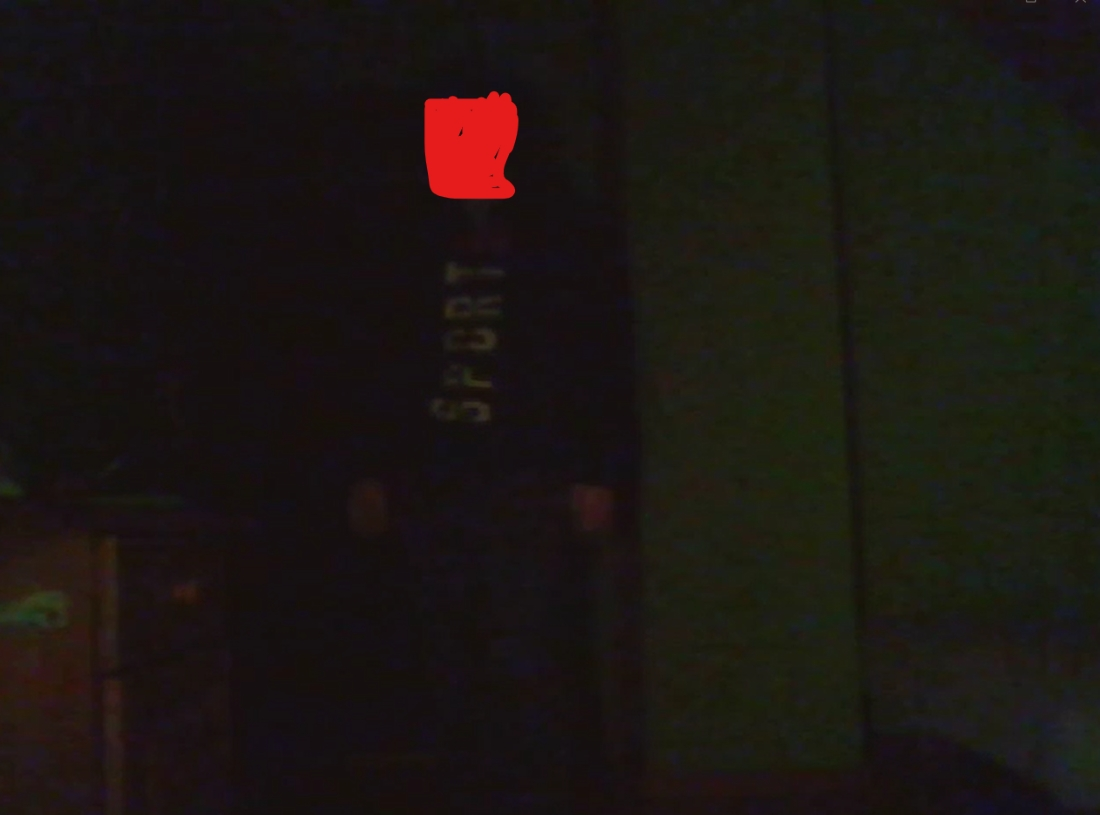
\includegraphics[width=\linewidth]{r_test_dokładności/vid_pics/4_2.jpg}
    \end{minipage}
    \caption{Poziomy oświetlenia dla filmów z obecnym człowiekiem}
    \label{fig:person_grid}
\end{figure}
\begin{figure}[H]
    \centering
    \begin{minipage}{0.45\textwidth}
        \centering
        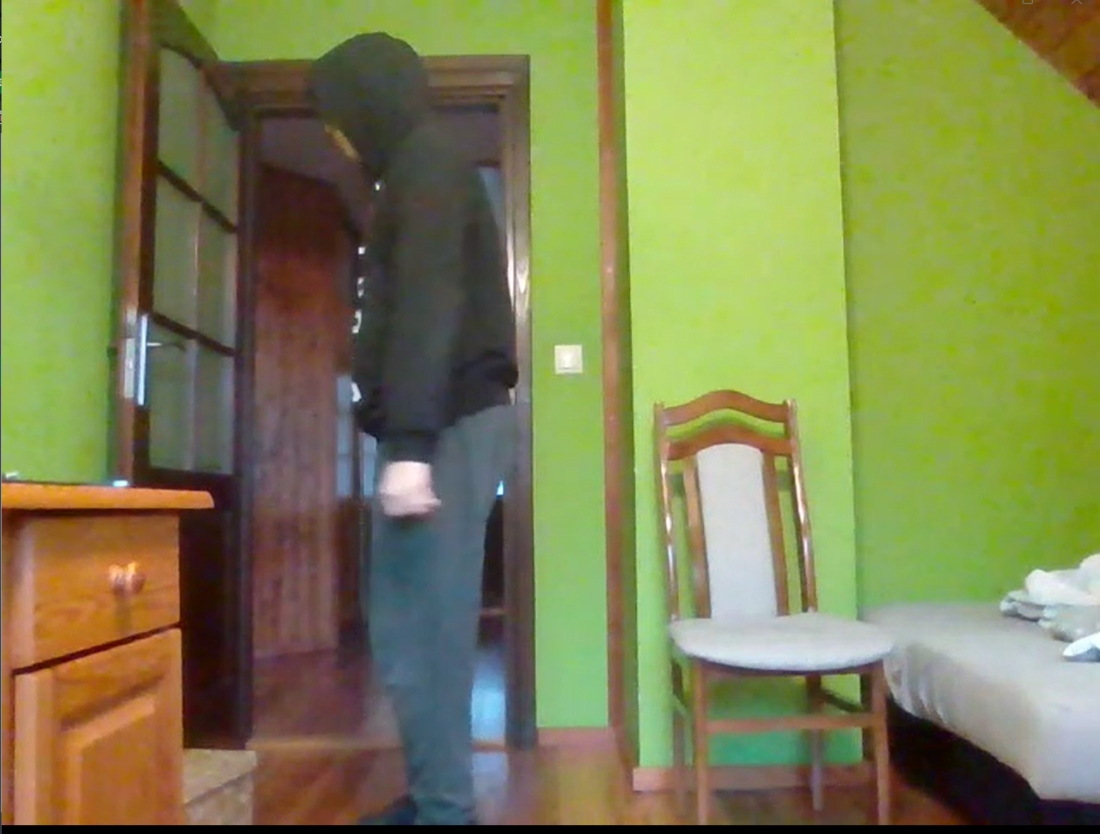
\includegraphics[width=\linewidth]{r_test_dokładności/vid_pics/1c_2.jpg}
    \end{minipage}\hfill
    \begin{minipage}{0.45\textwidth}
        \centering
        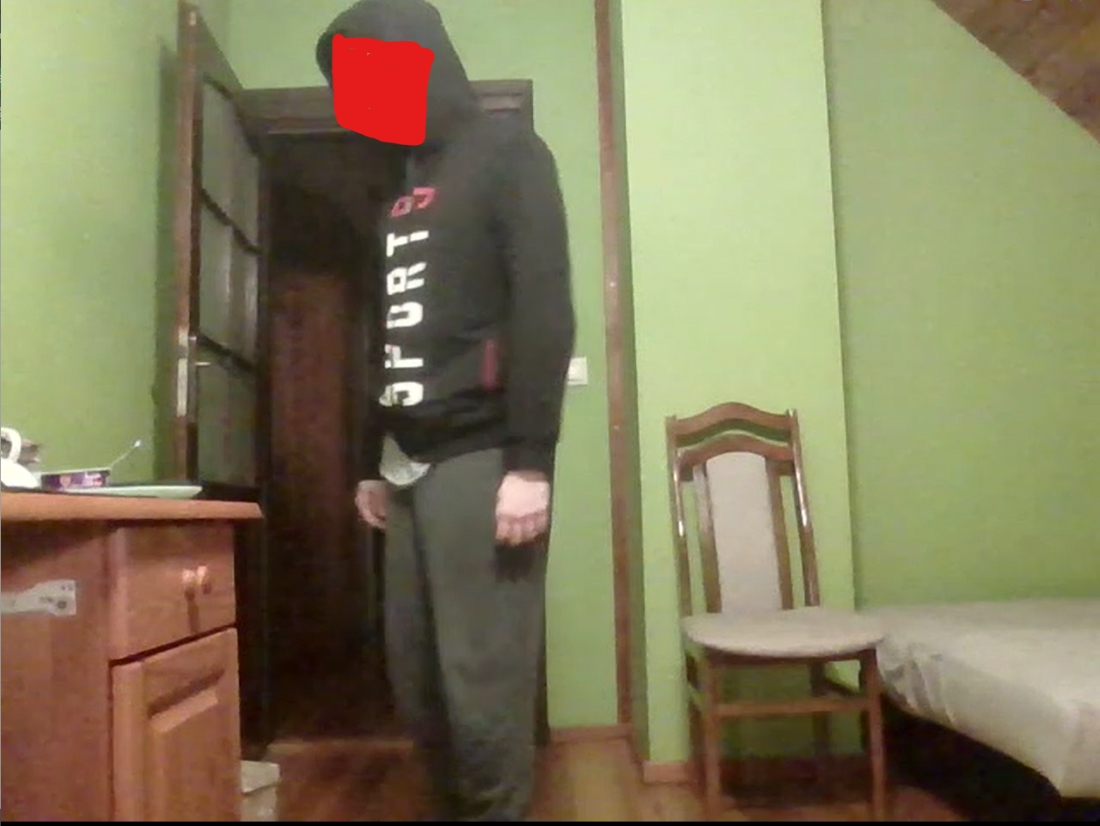
\includegraphics[width=\linewidth]{r_test_dokładności/vid_pics/2c_2.jpg}
    \end{minipage}
    \vskip\baselineskip
    \begin{minipage}{0.45\textwidth}
        \centering
        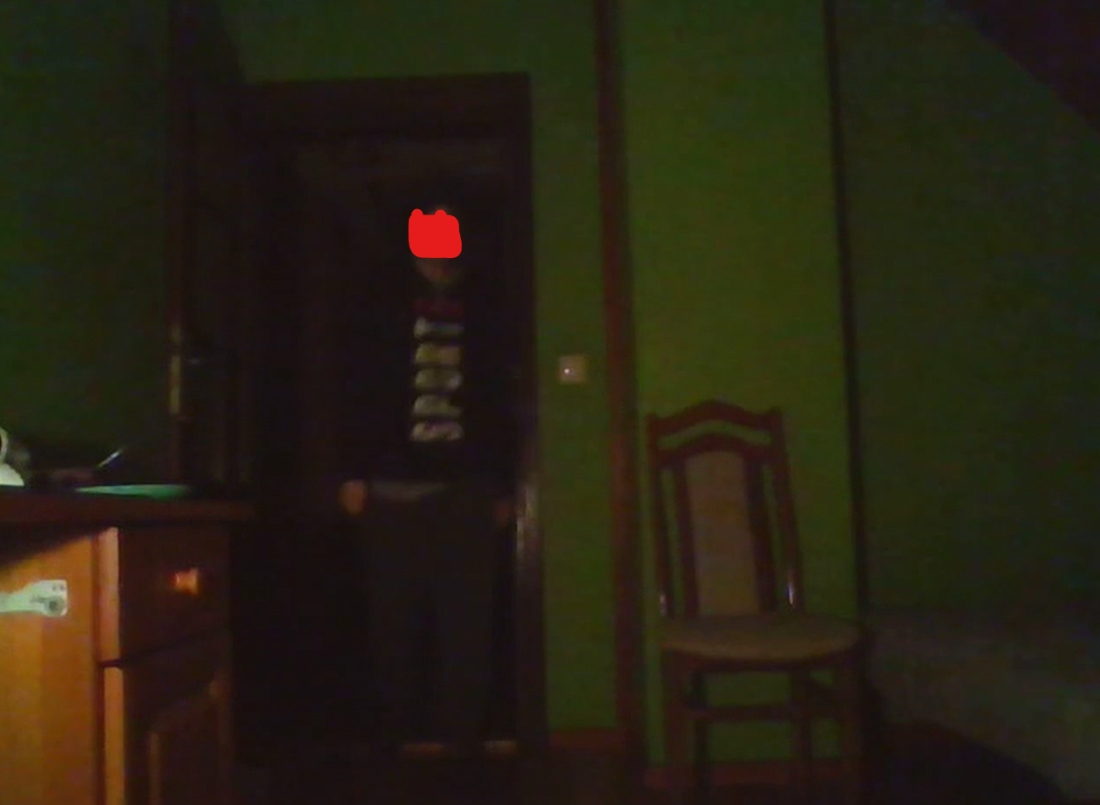
\includegraphics[width=\linewidth]{r_test_dokładności/vid_pics/3c_2.jpg}
    \end{minipage}\hfill
    \begin{minipage}{0.45\textwidth}
        \centering
        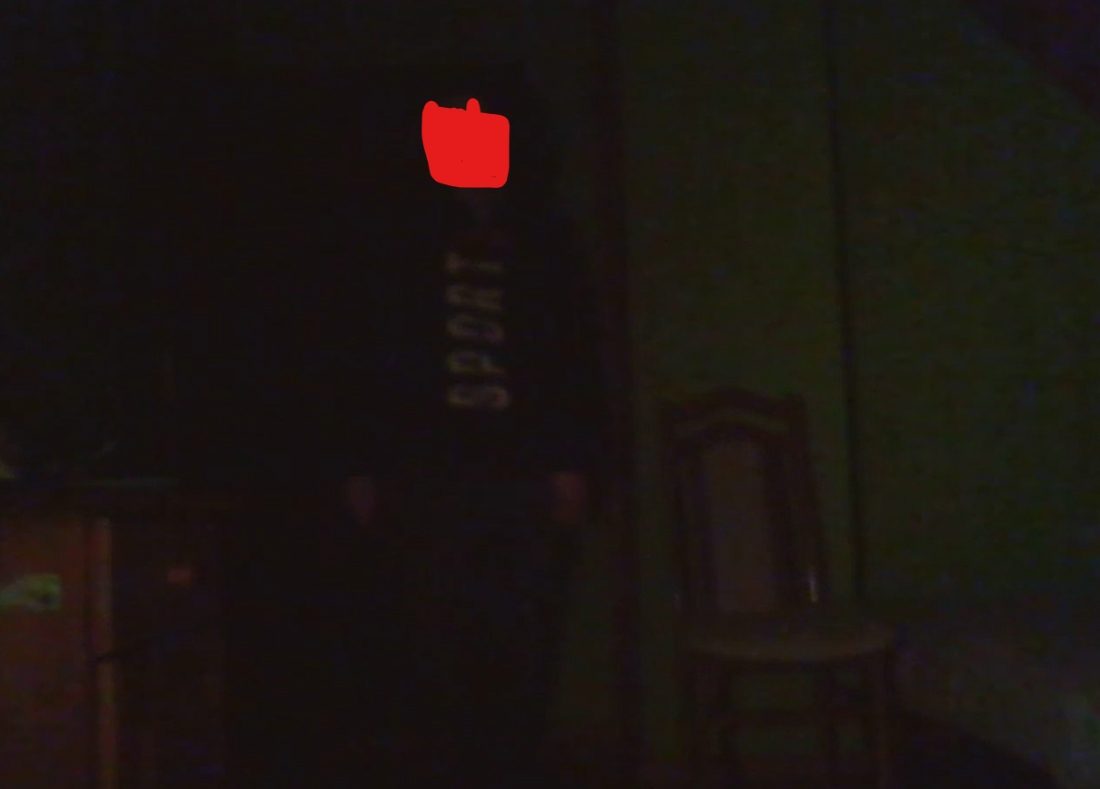
\includegraphics[width=\linewidth]{r_test_dokładności/vid_pics/4c_2.jpg}
    \end{minipage}
    \caption{Poziomy oświetlenia dla filmów z obecnym człowiekiem i krzesłem}
    \label{fig:chair_grid}
\end{figure}
\begin{figure}[H]
    \centering
    \begin{minipage}{0.45\textwidth}
        \centering
        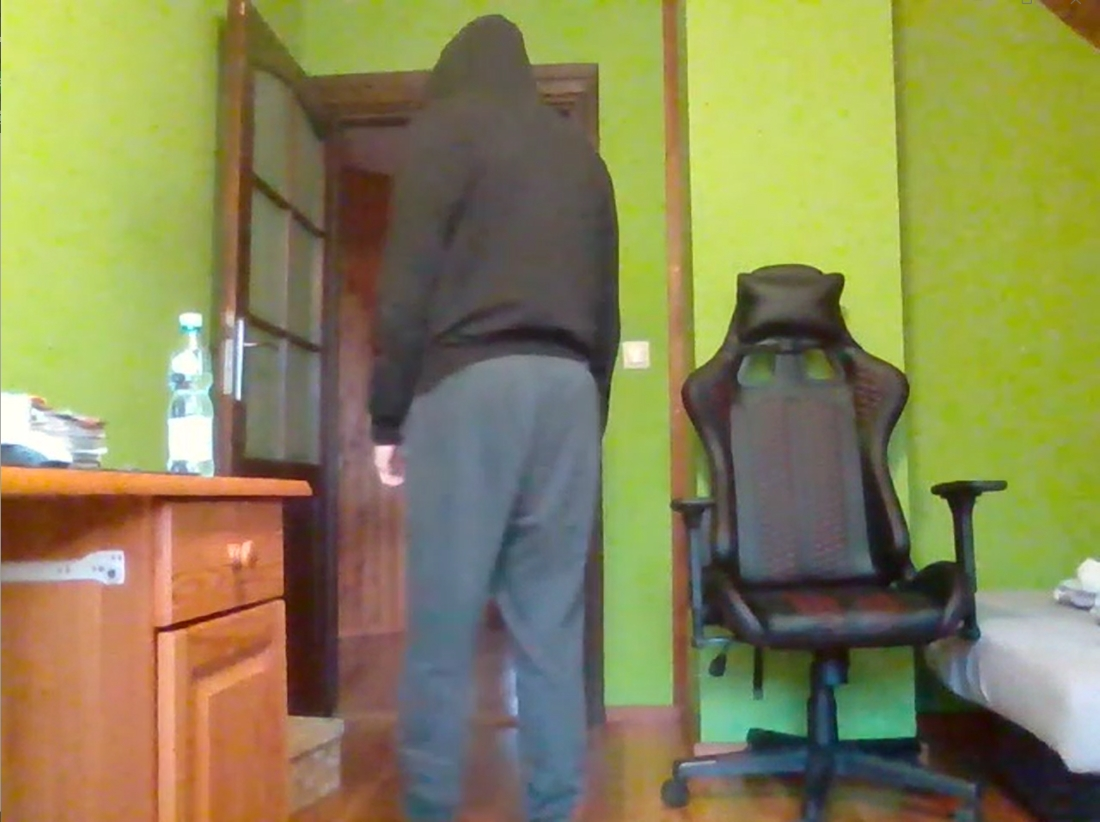
\includegraphics[width=\linewidth]{r_test_dokładności/vid_pics/1g_2.jpg}
    \end{minipage}\hfill
    \begin{minipage}{0.45\textwidth}
        \centering
        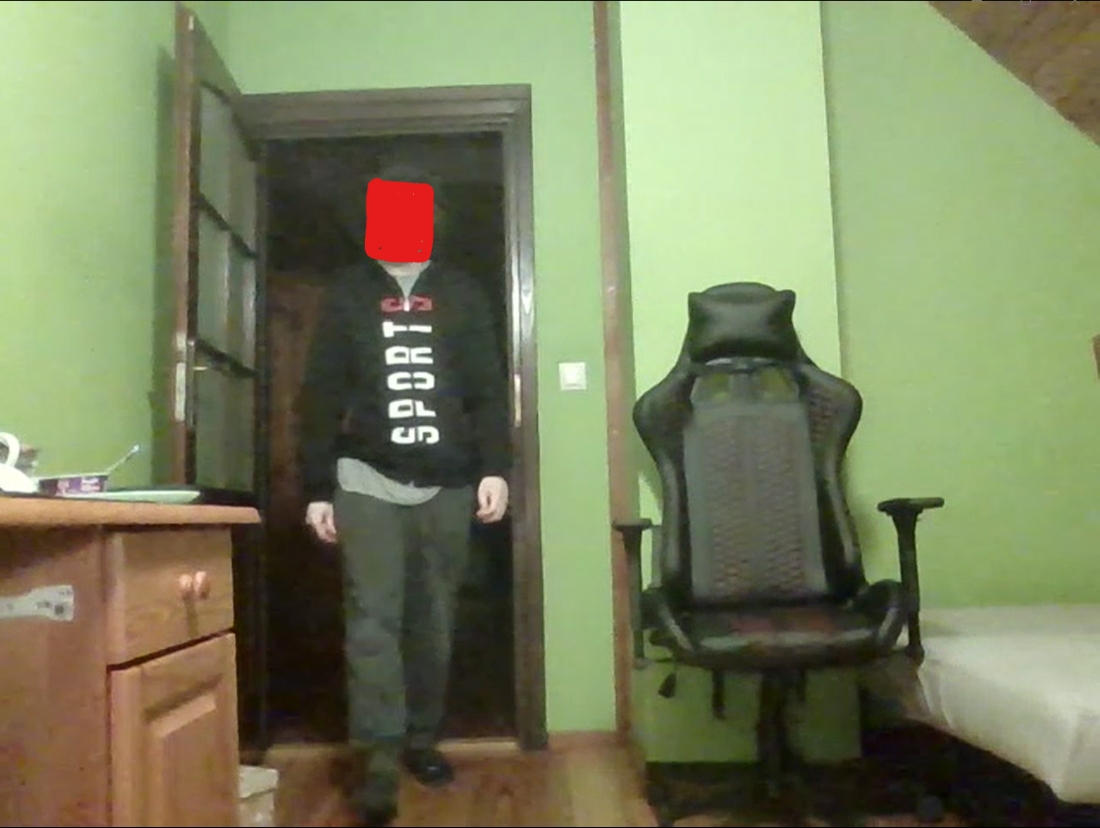
\includegraphics[width=\linewidth]{r_test_dokładności/vid_pics/2g_2.jpg}
    \end{minipage}
    \vskip\baselineskip
    \begin{minipage}{0.45\textwidth}
        \centering
        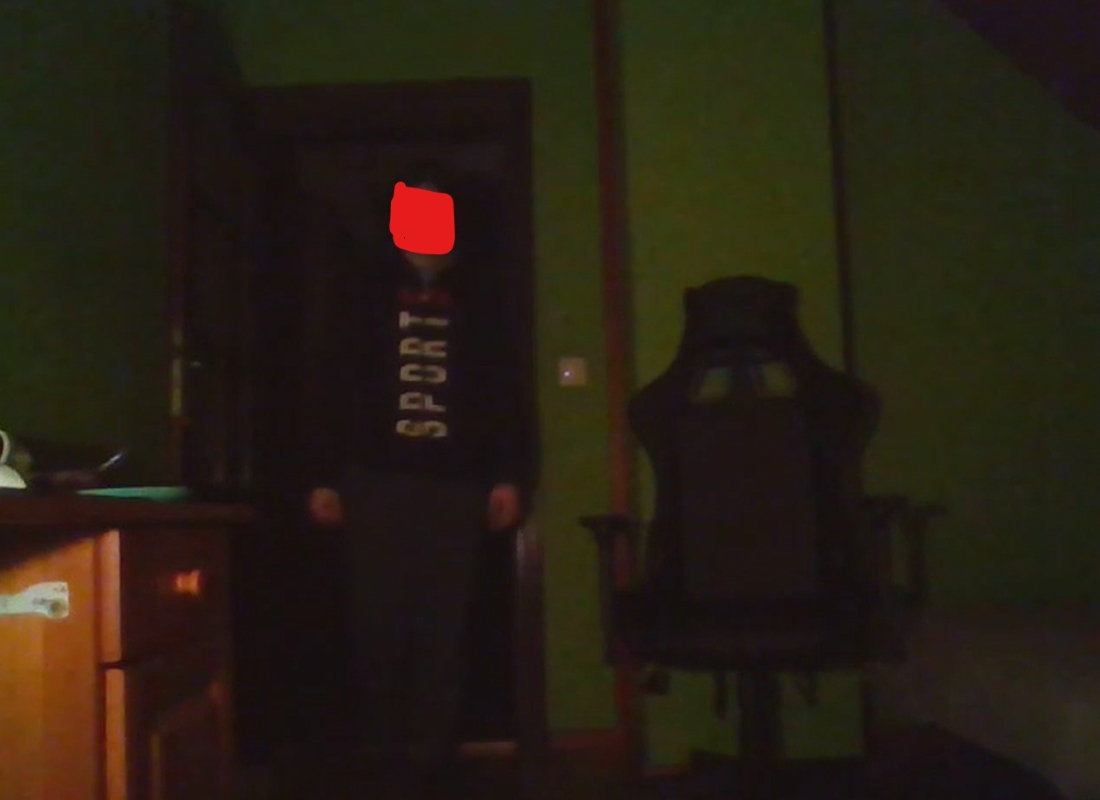
\includegraphics[width=\linewidth]{r_test_dokładności/vid_pics/3g_2.jpg}
    \end{minipage}\hfill
    \begin{minipage}{0.45\textwidth}
        \centering
        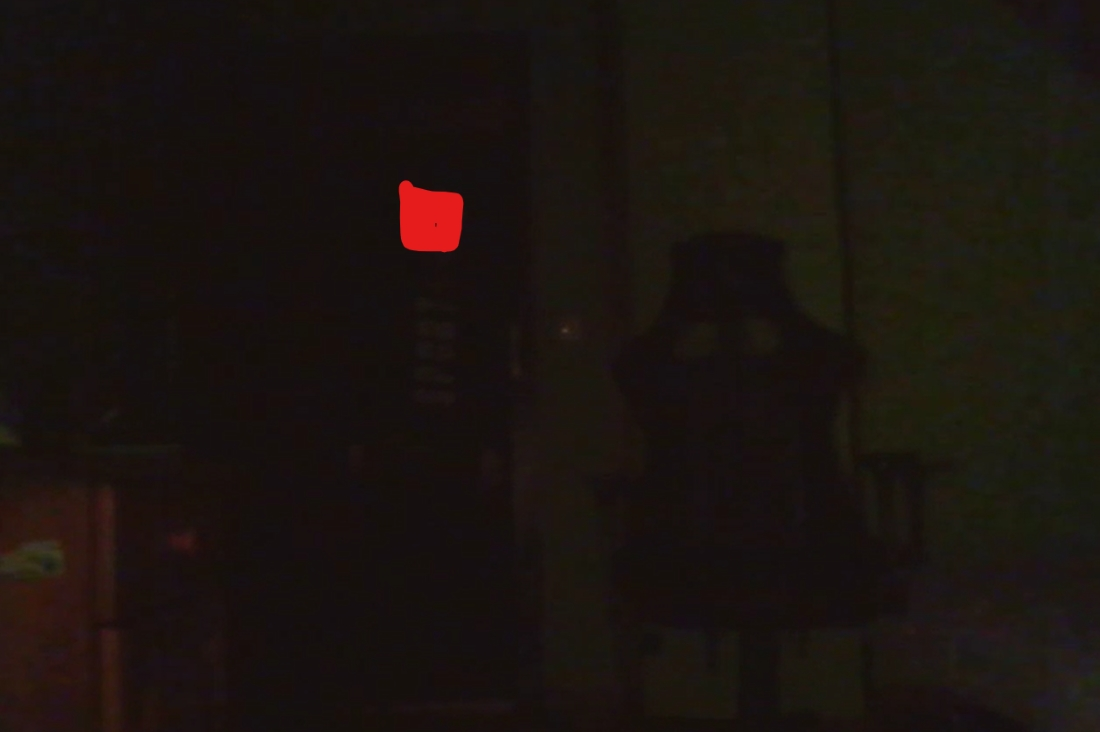
\includegraphics[width=\linewidth]{r_test_dokładności/vid_pics/4g_2.jpg}
    \end{minipage}
    \caption{Poziomy oświetlenia dla filmów z obecnym człowiekiem i fotelem}
    \label{fig:game_grid}
\end{figure}







\subsection{Metryki i dane wynikowe używane w testach}
Na podstawie opisanych dwunastu plików wideo wygenerowano dane do analizy w testach dla każdego z nich. Dane te to podstawowe metryki używane w klasyfikacji binarnej. Są to: wynik prawdziwy pozytywny (TP), wynik prawdziwy negatywny (TN), wynik fałszywy pozytywny (FP), wynik fałszywy negatywny (FN). 
Zaprojektowane testy sprawdzają tylko jedną klasę na test --- np. dla ewaluacji klasyfikacji klasy \emph{człowiek}, ignorowane są wykrycia innych klas. Co więcej, w niniejszym systemie nacisk kładziony jest na alarmowanie użytkownika o obecności obiektu, dlatego też uznano, iż więcej niż jedna detekcja klasy będzie przypisana do tej samej metryki co detekcja pojedynczego obiektu. 

Biorąc to pod uwagę, definicję metryk skonstruowano następująco: \\ \\ \noindent
Znaczenie skrótów z tabeli \ref{tab:saturation-value-table}: \\
$\emptyset$ -- brak wystąpienia obiektu wykrywanej klasy \\
x -- pojedyncze wystąpienie obiektu wykrywanej klasy \\
n*x -- wielokrotne wystąpienie obiektu wykrywanej klasy
\begin{table}[H]
    \centering
    \caption{Definicja metryk generowanych podczas testów detekcji obiektów.}
    \begin{tabular}{|>{\centering\arraybackslash}m{2cm}|>{\centering\arraybackslash}m{2cm}|>{\centering\arraybackslash}m{2.5cm}|>{\raggedright\arraybackslash}m{7.5cm}|}
    \hline
    Metryka & Obiekty na nagraniu & Obiekty wykryte przez detektor & \multicolumn{1}{c|}{Opis} \\ \hline



    \multirow{2}{*}{TP} & \multirow{2}{*}{x} & x & \multirow{2}{7.5cm}{Detektor wykrył jeden lub więcej obiektów klasy x, gdy obiekt x był obecny.} \\ \cline{3-3}

     &  & n*x & \\ \cline{1-4}



    TN & $\emptyset$ & $\emptyset$ & Detektor nie wykrył ani jednego obiektu klasy x, gdy obiekt x był nieobecny. \\ \hline

    

    \multirow{2}{*}{TN} & \multirow{2}{*}{$\emptyset$} & x & \multirow{2}{7.5cm}{Detektor wykrył jeden lub więcej obiektów klasy x, mimo że obiekt był nieobecny.} \\ \cline{3-3}

     &  & n*x & \\ \cline{1-4}



    FN & x & $\emptyset$ & Detektor nie wykrył ani jednego obiektu klasy x, mimo że obiekt był obecny. \\ \hline
    \end{tabular}
\end{table}

Generacja metryk wynikowych odbywa się w następująco:
\begin{enumerate}
    \item Wybierany jest film.
    \item Dla filmu metryki generowane są dla każdej badanej wartości progu ufności.
    \item Dla progu ufności analizowana jest każda klatka spełniająca wymagania opisane w rozdziale \ref{sec:zrodlo_wideo}. Dana klatka jest kategoryzowana do jednej z metryk.
    \item Metryka wynikowa to liczba klatek przypisanych do tej metryki.
\end{enumerate} 
Przykład wygenerowanych wyników prezentuje tabela \ref{tab:example-generated}.
\begin{table}[H]
    \centering
    \caption{Struktura wygenerowanych wyników na przykładzie częściowych wyników dla filmu z obecnym człowiekiem dla poziomu oświetlania nr 1. Wartości metryk to liczba klatek filmu przypisana do każdej z nich.}
    \begin{tabular}{ccccc}
    \hline
    \multicolumn{1}{|c|}{Próg   ufności} & \multicolumn{1}{c|}{TP}                    & \multicolumn{1}{c|}{TN}                    & \multicolumn{1}{c|}{FP}                    & \multicolumn{1}{c|}{FN}                    \\ \hline
    \multicolumn{1}{|c|}{0}                                 & \multicolumn{1}{c|}{100}                   & \multicolumn{1}{c|}{0}                     & \multicolumn{1}{c|}{122}                   & \multicolumn{1}{c|}{0}                     \\ \hline
    \multicolumn{1}{|c|}{0.01}                              & \multicolumn{1}{c|}{100}                   & \multicolumn{1}{c|}{49}                    & \multicolumn{1}{c|}{73}                    & \multicolumn{1}{c|}{0}                     \\ \hline
    \multicolumn{1}{|c|}{0.02}                              & \multicolumn{1}{c|}{100}                   & \multicolumn{1}{c|}{104}                   & \multicolumn{1}{c|}{18}                    & \multicolumn{1}{c|}{0}                     \\ \hline
    \multicolumn{1}{|c|}{0.03}                              & \multicolumn{1}{c|}{100}                   & \multicolumn{1}{c|}{120}                   & \multicolumn{1}{c|}{2}                     & \multicolumn{1}{c|}{0}                     \\ \hline
    \multicolumn{1}{|c|}{0.04}                              & \multicolumn{1}{c|}{100}                   & \multicolumn{1}{c|}{122}                   & \multicolumn{1}{c|}{0}                     & \multicolumn{1}{c|}{0}                     \\ \hline
    \multicolumn{5}{c}{$\bullet$ $\bullet$   $\bullet$ $\bullet$ $\bullet$ $\bullet$ $\bullet$ $\bullet$ $\bullet$   $\bullet$ $\bullet$ $\bullet$ $\bullet$ $\bullet$ $\bullet$ $\bullet$   $\bullet$ $\bullet$ $\bullet$ $\bullet$ $\bullet$} \\ \hline
    \multicolumn{1}{|c|}{0.96}                              & \multicolumn{1}{c|}{0}                     & \multicolumn{1}{c|}{122}                   & \multicolumn{1}{c|}{0}                     & \multicolumn{1}{c|}{100}                   \\ \hline
    \multicolumn{1}{|c|}{0.97}                              & \multicolumn{1}{c|}{0}                     & \multicolumn{1}{c|}{122}                   & \multicolumn{1}{c|}{0}                     & \multicolumn{1}{c|}{100}                   \\ \hline
    \multicolumn{1}{|c|}{0.98}                              & \multicolumn{1}{c|}{0}                     & \multicolumn{1}{c|}{122}                   & \multicolumn{1}{c|}{0}                     & \multicolumn{1}{c|}{100}                   \\ \hline
    \multicolumn{1}{|c|}{0.99}                              & \multicolumn{1}{c|}{0}                     & \multicolumn{1}{c|}{122}                   & \multicolumn{1}{c|}{0}                     & \multicolumn{1}{c|}{100}                   \\ \hline
    \multicolumn{1}{|c|}{1}                                 & \multicolumn{1}{c|}{0}                     & \multicolumn{1}{c|}{122}                   & \multicolumn{1}{c|}{0}                     & \multicolumn{1}{c|}{100}                   \\ \hline
    \end{tabular}
    \label{tab:example-generated}
    \end{table}


\section{Test dokładności pojedyńczej klasy}
\label{sec:test-1}
Niniejszy podrozdział przedstawia różne badania, których celem jest ewaluacja klasyfikacji YOLOv8n na przykładzie klasy człowiek. Model zbadano pod kątem wpływu jak manipulacja poziomem oświetlenia oraz progu ufności przekłada się na jego wyniki. Dla każdego zmierzonego progu ufności wyznaczane będą metryki potrzebne do zobrazowania wniosków. Będą one liczone na podstawie poprzednio uzyskanych metryk --- TP, TN, FP i FN. Do testu wykrzystano cztery filmy. Każdy z nich przedstawia wyłącznie człowieka. Wartości jasności i nasycenia przedstawiono w tabeli \ref{tab:saturacja-jasnosc-czlowiek}. Wygląd nagranego pomieszczenia dla różnych poziomów oświetlenia ukazano na rysunku \ref{fig:person_grid}. 

\begin{table}[H]
\centering
\caption{Jasność i nasycenie dla wszystkich filmów.}
\begin{tabular}{|c|c|c|c|}
\hline
Poziom oświetlenia  & Obecne obiekty & Jasność & Nasycenie \\ \hline
1        & człowiek       & 152.73  & 107.3     \\ \hline
2        & człowiek       & 134.64  & 93.48     \\ \hline
3        & człowiek       & 41.59   & 123.48    \\ \hline
4        & człowiek       & 25.47   & 90.92     \\ \hline
\end{tabular}

\label{tab:saturacja-jasnosc-czlowiek}
\end{table}


\subsection{Ewaluacja modelu dla różnych poziomów oświetlenia}
\label{sec:test-AUC}
W celu zobrazowania i oceniania wyniku modelu zastosowano metrykę 

\begin{figure}[H]
    \centering
    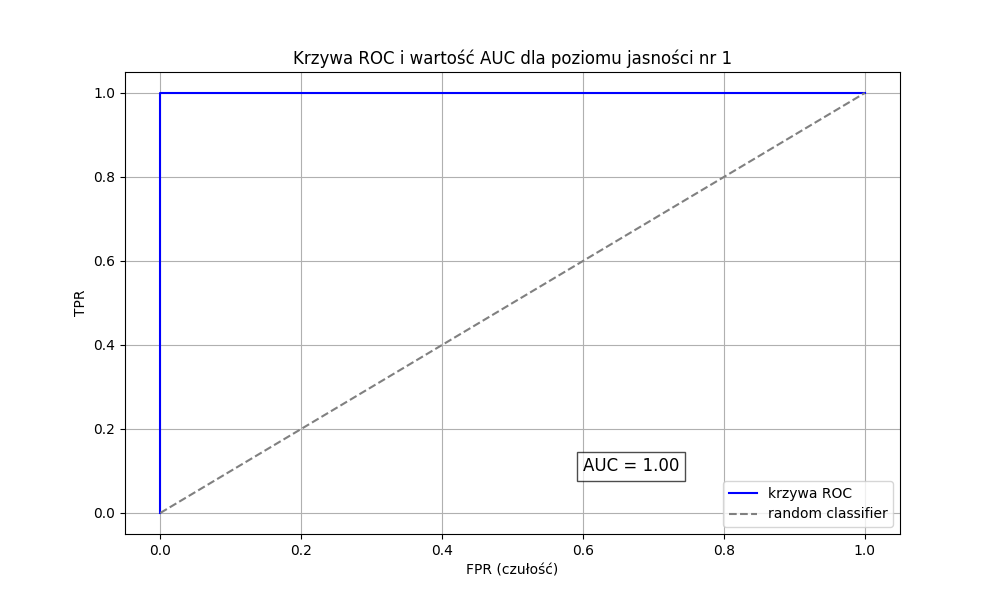
\includegraphics[width=\linewidth]{r_test_dokładności/AUC_charts/1.png}
    \caption{Krzywa ROC i wartość AUC dla poziomu jasności nr 1.}
    \label{fig:ROC-1}
\end{figure}

\begin{figure}[H]
    \centering
    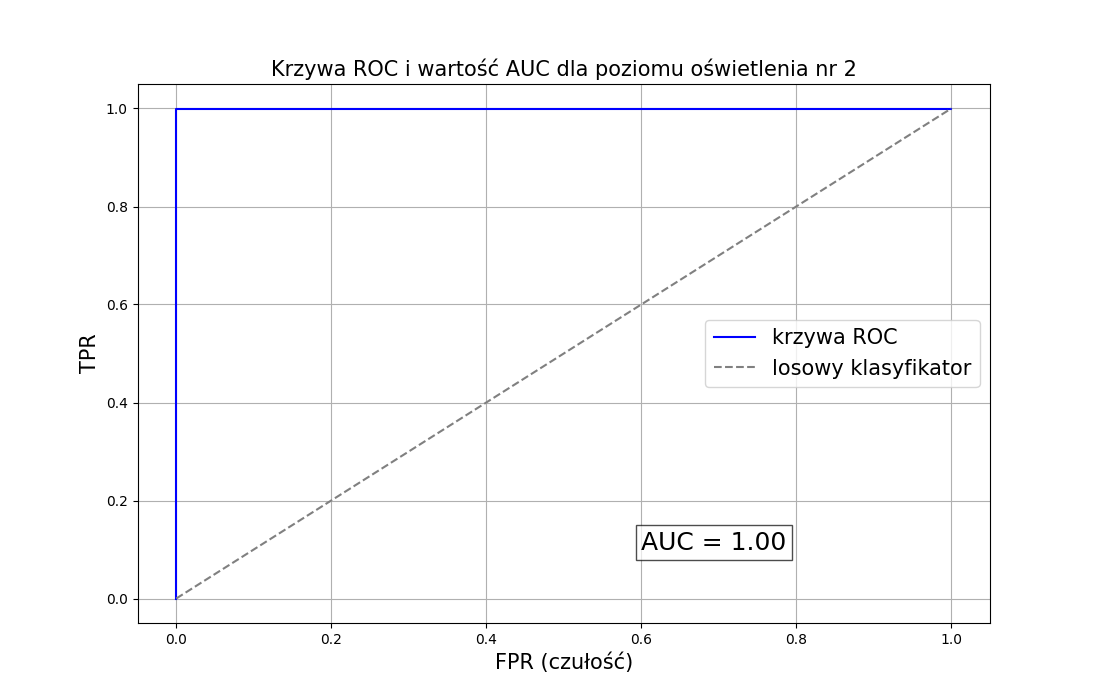
\includegraphics[width=\linewidth]{r_test_dokładności/AUC_charts/2.png}
    \caption{Krzywa ROC i wartość AUC dla poziomu jasności nr 2.}
    \label{fig:ROC-2}
\end{figure}

\begin{figure}[H]
    \centering
    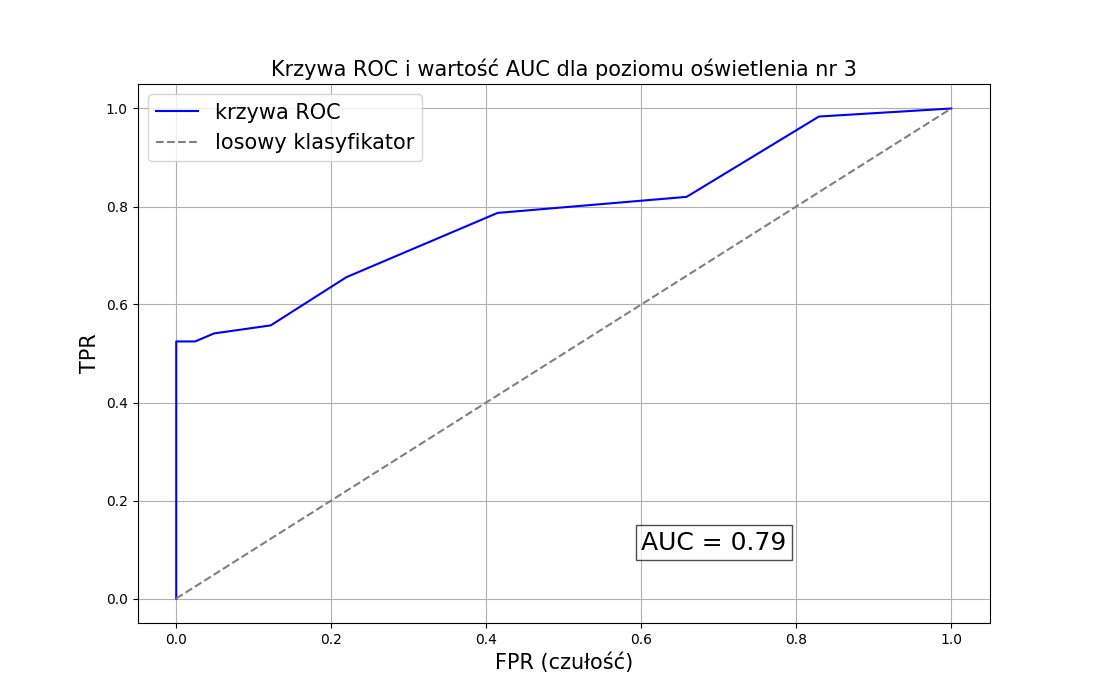
\includegraphics[width=\linewidth]{r_test_dokładności/AUC_charts/3.png}
    \caption{Krzywa ROC i wartość AUC dla poziomu jasności nr 3.}
    \label{fig:ROC-3}
\end{figure}

\begin{figure}[H]
    \centering
    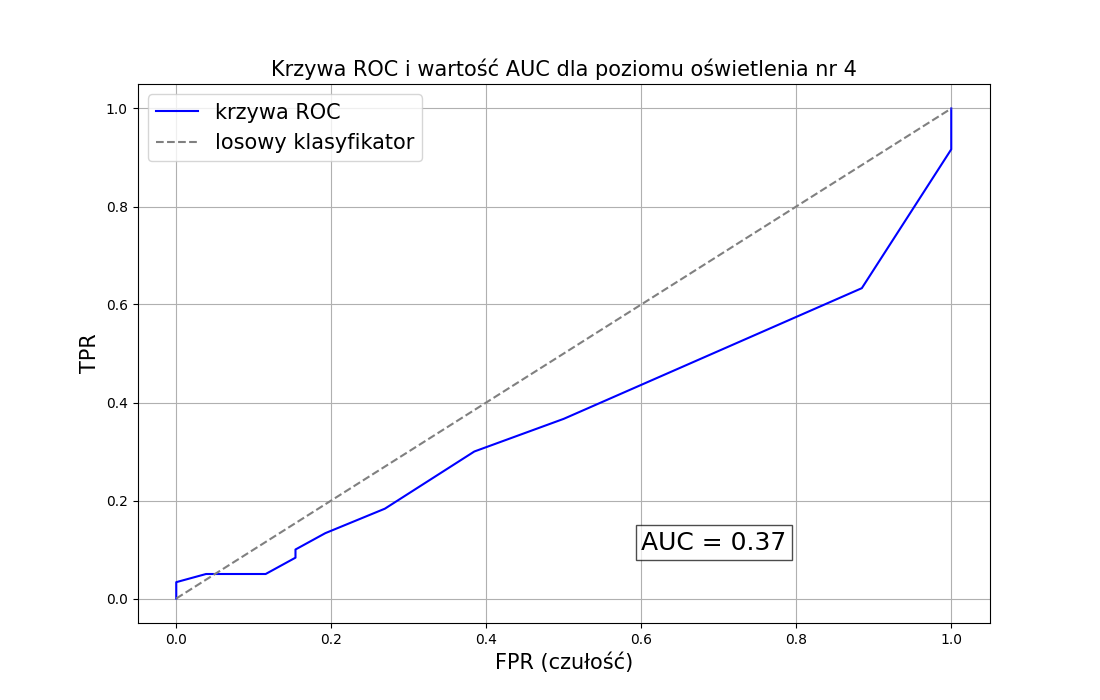
\includegraphics[width=\linewidth]{r_test_dokładności/AUC_charts/4.png}
    \caption{Krzywa ROC i wartość AUC dla poziomu jasności nr 4.}
    \label{fig:ROC-4}
\end{figure}

\begin{figure}[H]
    \centering
    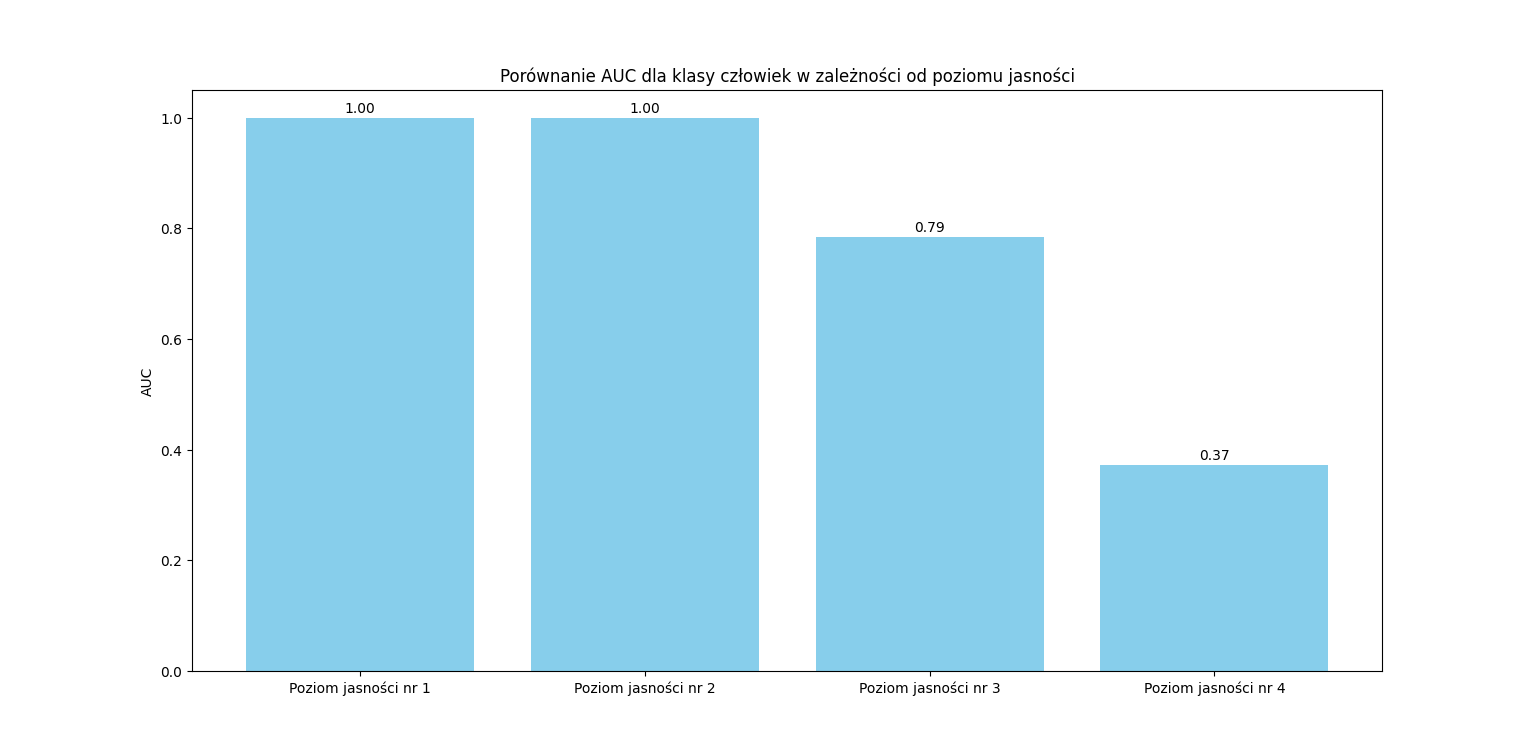
\includegraphics[width=\linewidth]{r_test_dokładności/AUC_charts/porownanieAUC.png}
    \caption{Wykres porównujący wartości AUC dla zbadanych poziomów jasności.}
    \label{fig:AUC}
\end{figure}



\subsection{Analiza wpływu progu ufności na wyniki detekcji}



\section{Test poziomu generalizacji modelu}
\label{sec:test-2}
W tej sekcji zbadano jak dobrze model radzi sobie z różnymi obiektami należącymi do tej samej klasy. Umiejętność generalizacji zostanie sprawdzona na przykładzie klasy \emph{krzesło} (ang. \emph{chair}). Użyte obiekty to krzesło oraz fotel dla graczy (dalej zwany fotelem). Nazwy angielskie tych obiektów to kolejno \emph{chair} i \emph{gaming chair}, jest to ważne, ponieważ klasy COCO zostały stworzone według angielskiego nazwenictwa, na którego podstawie przypisuje się rózne warianty obiektów do jednej klas.  W badaniu tym porównano wyniki dla krzesła i fotela w funkcji progu ufności dla wszystkich (czterech) poziomów ośwetlenia. Do testu wykorzystano osiem filmów -- cztery z widocznym krzesłem i człowiekiem, cztery z widocznym fotelem i człowiekiem. Wartości jasności i nasycenia dla każdego filmu ukazono w tabeli \ref{tab:jasnosc-krzeslo-fotel}. Wygląd nagranego pomieszczenia wraz z nagranym obiektem dla różnych poziomów oświetlenia ukazano na rysunku \ref{fig:chair_grid} (człowiek, krzesło) i 
\ref{fig:game_grid} (człowiek fotel). 
% Please add the following required packages to your document preamble:
% \usepackage{multirow}
\begin{table}[H]
    \centering
    \caption{Jasność i nasycenie dla wszystkich filmów. Pogrubiona czcionka oznacza obiekt należący do analizowanej klasy.}
    \begin{tabular}{|c|c|c|c|}
    \hline
    Poziom   oświetlenia & Obecne obiekty                                & Jasność & Nasycenie \\ \hline
    \multirow{2}{*}{1}   & człowiek,   
    \textbf{krzesło} & 149.92  & 119.07    \\ \cline{2-4} 
                         & człowiek, \textbf{fotel}     & 152.68  & 111.47    \\ \hline
    \multirow{2}{*}{2}   & człowiek,   \textbf{krzesło} & 139.14  & 90.71     \\ \cline{2-4} 
                         & człowiek, \textbf{fotel}     & 133.77  & 83.29     \\ \hline
    \multirow{2}{*}{3}   & człowiek,   \textbf{krzesło} & 38.91   & 132.31    \\ \cline{2-4} 
                         & człowiek, \textbf{fotel}     & 38.12   & 124.31    \\ \hline
    \multirow{2}{*}{4}   & człowiek,   \textbf{krzesło} & 25.3    & 100.8     \\ \cline{2-4} 
                         & człowiek, \textbf{fotel}     & 24.88   & 108.5     \\ \hline
    \end{tabular}
    \label{tab:jasnosc-krzeslo-fotel}
    \end{table}

Tak jak to wspomniano (podrozdział \ref{sec:zrodlo_wideo}), badane obiekty są statyczne i były obecne przez wszystkie klatki każdego filmu. Dlatego też metryki FP i TN są zawsze zerowe. Do tego badania można jednak ponownie skorzystać z TPR, ponieważ metryka ta bazuje jedynie na TP i FN. TPR jest alternatywnie nazywane czułościa i to badanie tak będzie się do niej odwoływać. Czułość dla fotela i krzesła jest zestawiona w funkcji progu ufności dla kolejnych poziomów oświetlenia (wykresy na rysnkach \ref{fig:chair-game-1}, \ref{fig:chair-game-2}, \ref{fig:chair-game-3}, \ref{fig:chair-game-4}). Porównano również poziomy oświetlenia dla konkretnego obiektu -- \ref{fig:all_bright_chair} (krzesło), \ref{fig:all_bright_game} (fotel). 

Wyniki dla każdego poziomu oświetlenia okazały się być lepsze dla krzesła. Przyczyn można upatrywać w dwóch źródłach: po pierwsze, zdecydowanie ciemniejszy kolor fotela jest ciężej wykrywany w coraz ciemniejszym pomieszczeniu. Po drugie, model COCO mógł być wytrenowany dla mniejszej liczby foteli tego typu.

Odnośnie przyczyny pierwszej, można dostrzec zauważalny spadek skuteczeności klasyfikacji na niższych poziomach oświetlenia od poziomu 1. Stało sie tak, pomimo że poziom 2 został uznany za poziom dobrej widoczności -- fotel jest wyraźnie wyszczególniony. Przyczyną może być np. niska jakość nagranego filmu, w tym zakłócenia. 

Podsumowując, stwierdzono, iż model nie generalizuje dobrze klasy \emph{krzesło}. Samo badanie nie świadczy, iż generalizacja YOLOv8n ma podobną jakość w przypadku innych klas. Interesującym rozszerzeniem badań byłoby zbadanie klas niestetycznych, czego nie udało się zrealizować przez wzgląd na osobisty brak takich obiektów. 

\begin{figure}[H]
    \centering
    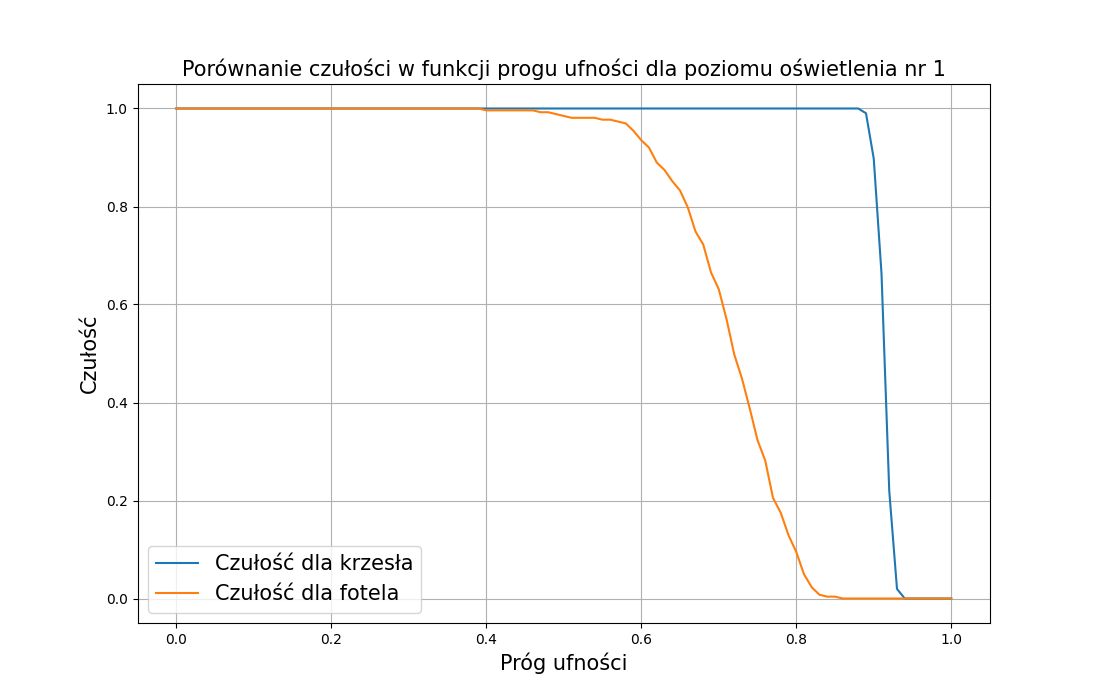
\includegraphics[width=\linewidth]{r_test_dokładności/chair_charts/1.png}
    \caption{Porównanie czułości w funkcji progu ufności dla krzesła i fotela. Poziom oświetlania nr 1.}
    \label{fig:chair-game-1}
\end{figure}

\begin{figure}[H]
    \centering
    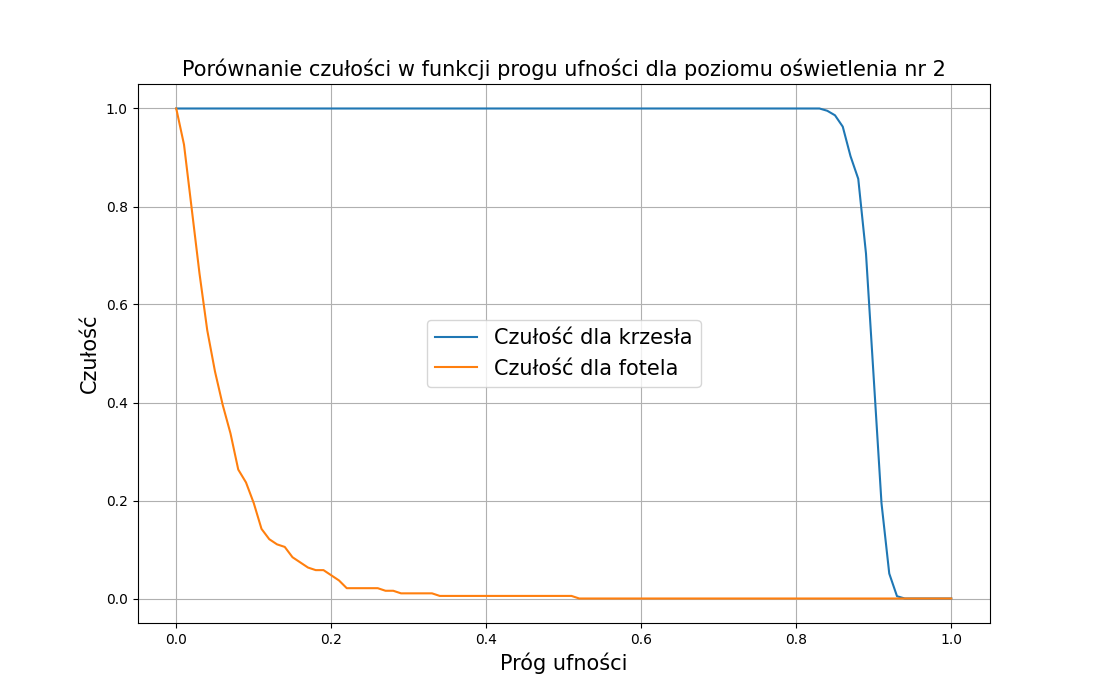
\includegraphics[width=\linewidth]{r_test_dokładności/chair_charts/2.png}
    \caption{Porównanie czułości w funkcji progu ufności dla krzesła i fotela. Poziom oświetlania nr 2.}
    \label{fig:chair-game-2}
\end{figure}

\begin{figure}[H]
    \centering
    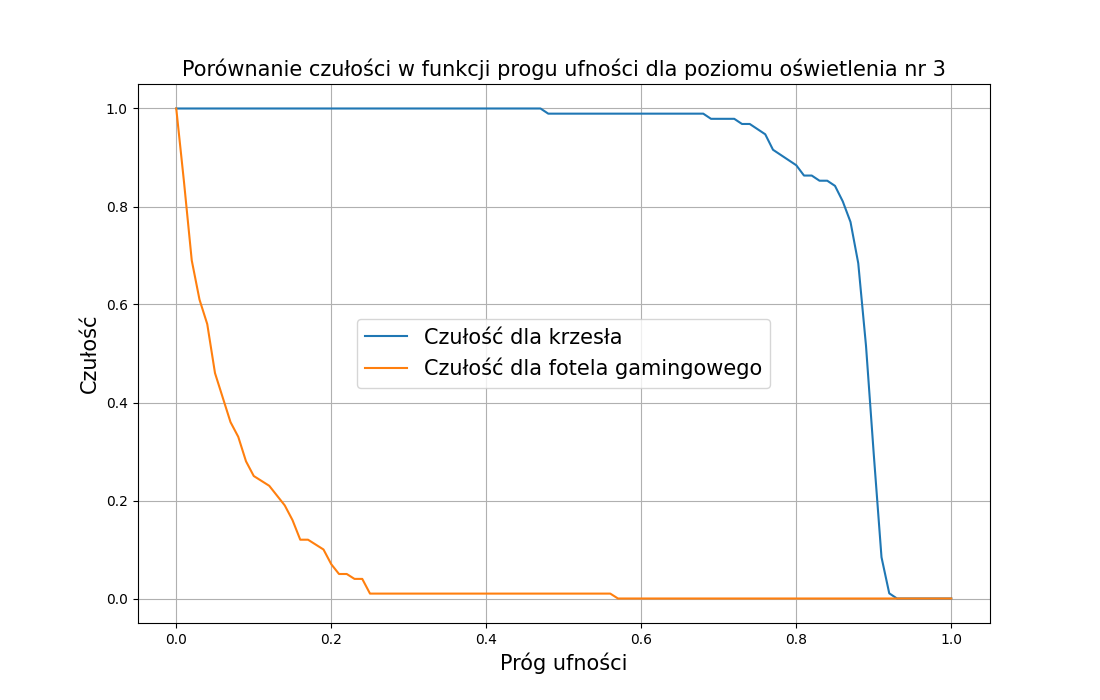
\includegraphics[width=\linewidth]{r_test_dokładności/chair_charts/3.png}
    \caption{Wykres do porównania czułości w funkcji progu ufności dla krzesła i fotela. Poziom oświetlania nr 3.}
    \label{fig:chair-game-3}
\end{figure}

\begin{figure}[H]
    \centering
    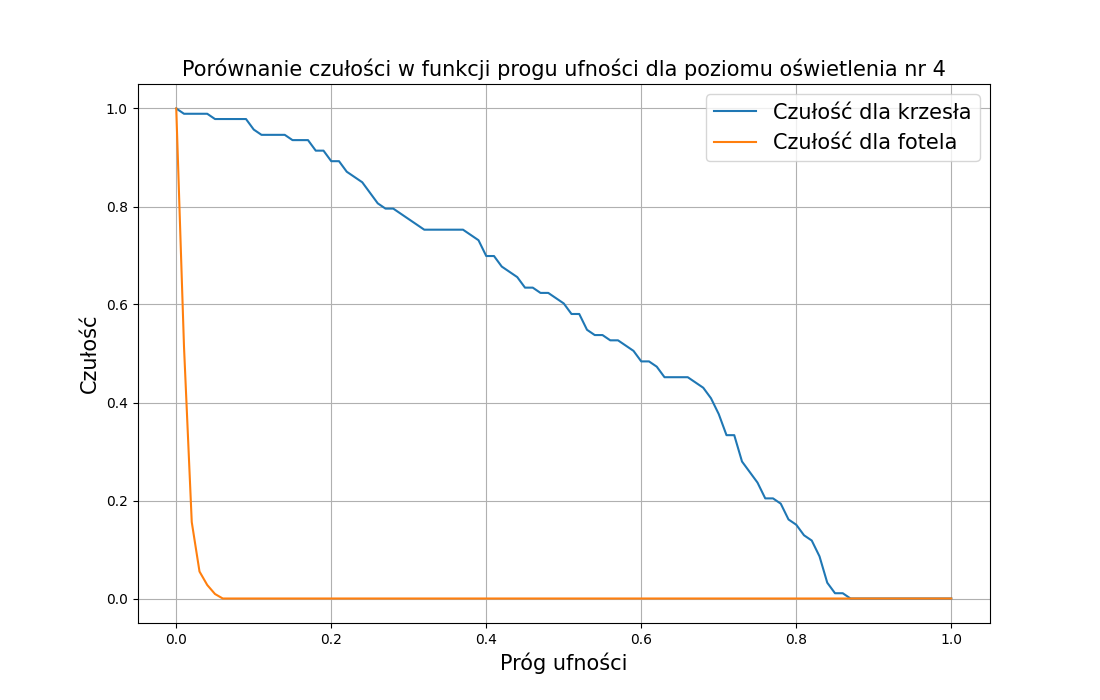
\includegraphics[width=\linewidth]{r_test_dokładności/chair_charts/4.png}
    \caption{Wykres do porównania czułości w funkcji progu ufności dla krzesła i fotela. Poziom oświetlania nr 4.}
    \label{fig:chair-game-4}
\end{figure}

\begin{figure}[H]
    \centering
    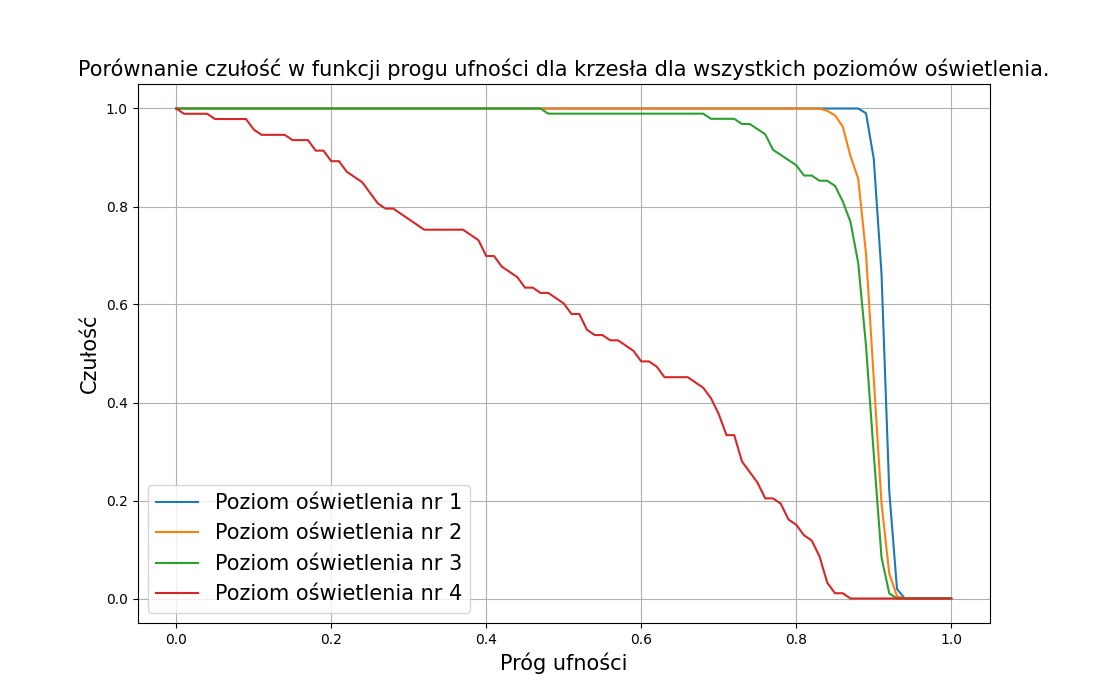
\includegraphics[width=\linewidth]{r_test_dokładności/chair_charts/chair.png}
    \caption{Wykres do porównania czułości w funkcji progu ufności dla wszystkich poziomów oświetlania. Obiekt --  krzesło.}
    \label{fig:all_bright_chair}
\end{figure}

\begin{figure}[H]
    \centering
    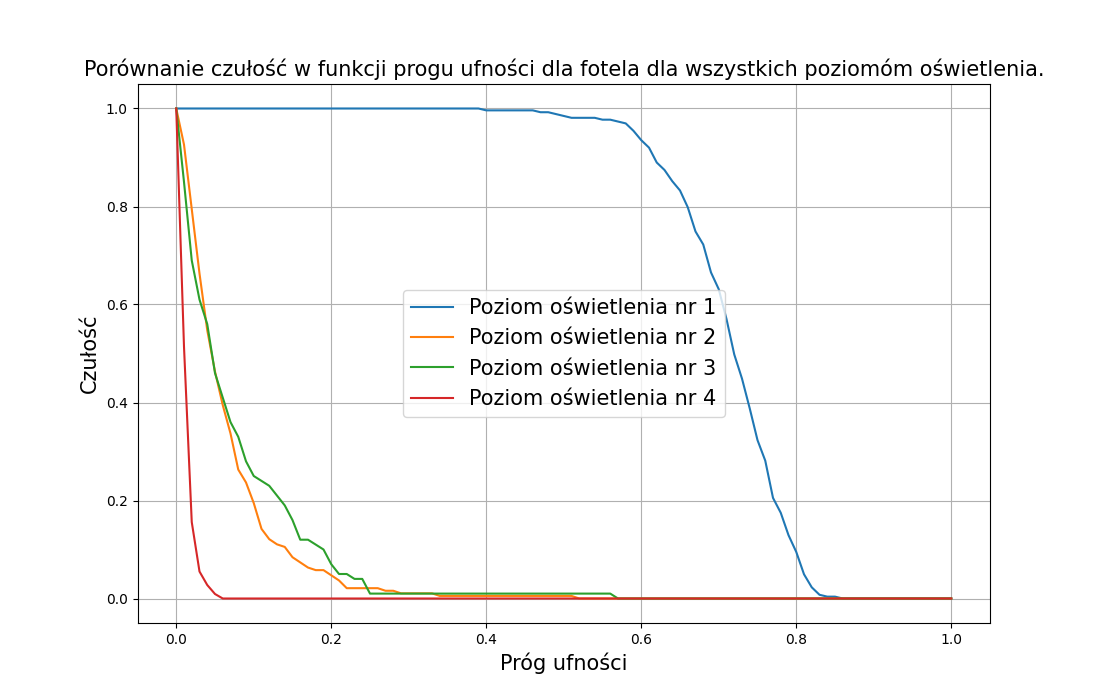
\includegraphics[width=\linewidth]{r_test_dokładności/chair_charts/gaming-chair.png}
    \caption{Wykres do porównania czułości w funkcji progu ufności dla wszystkich poziomów oświetlania. Obiekt --  fotel.}
    \label{fig:all_bright_game}
\end{figure}

